\documentclass[12pt]{article}
\usepackage[paper=letterpaper,margin=2cm]{geometry}
\usepackage{amsmath,amssymb,amsfonts}
\usepackage{newtxtext,newtxmath}
\usepackage{enumitem}
\usepackage{titling}
\usepackage{subfig,graphicx}
\usepackage[colorlinks=true]{hyperref}
\usepackage{multirow}
\usepackage{listings}
\usepackage[dvipsnames]{xcolor}
\usepackage{float}

\newcommand{\ind}{\perp\!\!\!\perp}

\definecolor{codegreen}{rgb}{0,0.6,0}
\definecolor{codegray}{rgb}{0.5,0.5,0.5}
\definecolor{codepurple}{rgb}{0.58,0,0.82}

% BACKGROUND BOX COLORS
\definecolor{byellow}{HTML}{e0b400}
\definecolor{bmint}{HTML}{00c49a}

% \highlight[<colour>]{<stuff>}
\newcommand{\highlight}[2][yellow]{\mathchoice
  {\colorbox{#1}{$\displaystyle#2$}}
  {\colorbox{#1}{$\textstyle#2$}}
  {\colorbox{#1}{$\scriptstyle#2$}}
  {\colorbox{#1}{$\scriptscriptstyle#2$}}}

\lstdefinestyle{mystyle}{
    commentstyle=\color{codegreen},
    keywordstyle=\color{magenta},
    numberstyle=\tiny\color{codegray},
    stringstyle=\color{codepurple},
    basicstyle=\ttfamily\footnotesize,
    breakatwhitespace=false,
    breaklines=true,
    captionpos=b,
    keepspaces=true,
    numbers=left,
    numbersep=6pt,
    showspaces=false,
    showstringspaces=false,
    showtabs=false,
    tabsize=2
}
\lstset{style=mystyle}

\begin{document}
\begin{center}
\large{Aprendizagem 2023} \\
Homework IV -- Group 28 \\
\vskip 0.3cm
Gonçalo Bárias (ist1103124) \& Raquel Braunschweig (ist1102624)\vskip 1cm

\large{\textbf{Part I}: Pen and Paper}\normalsize
\end{center}

\noindent Given the following observations, $\left\{\begin{pmatrix} 1 \\ 0.6 \\ 0.1 \end{pmatrix}, \begin{pmatrix} 0 \\ -0.4 \\ 0.8 \end{pmatrix}, \begin{pmatrix} 0 \\ 0.2 \\ 0.5 \end{pmatrix},
\begin{pmatrix} 1 \\ 0.4 \\ -0.1 \end{pmatrix}\right\}$.

\vskip 0.2cm
\noindent Consider a Bayesian clustering that assumes $\{y_1\} \ind \{y_2, y_3\}$, two clusters following a Bernoulli distribution on $y_1$ ($p_1$ and $p_2$), a multivariate Gaussian on $\{y_2, y_3\}$ ($N_1$ and $N_2$),
and the following initial mixture:

\vskip -0.3cm
\begin{equation*}
    \pi_1 = 0.5 \quad , \quad \pi_2 = 0.5
\end{equation*}
\begin{equation*}
    p_1 = P(y_1 = 1) = 0.3 \quad , \quad p_2 = P(y_1 = 1) = 0.7
\end{equation*}
\begin{equation*}
    \mathcal{N}_1 \left(\boldsymbol{\mu}_1 = \begin{pmatrix} 1 \\ 1 \end{pmatrix}, \mathbf{\Sigma}_1 = \begin{pmatrix} 2 & 0.5 \\ 0.5 & 2 \end{pmatrix}\right) \quad
    , \quad \mathcal{N}_2 \left(\boldsymbol{\mu}_2 = \begin{pmatrix} 0 \\ 0 \end{pmatrix}, \mathbf{\Sigma}_2 = \begin{pmatrix} 1.5 & 1 \\ 1 & 1.5 \end{pmatrix}\right)
\end{equation*}

\vskip 0.2cm
\begin{enumerate}[leftmargin=\labelsep]
    \item \textbf{Perform one epoch of the EM clustering algorithm and determine the new parameters.}\\
          \textbf{\textit{Hint:} we suggest you to use numpy and scipy, however disclose the intermediary results step by step.}

          \vskip 0.3cm
          The EM (Expectation-Maximization) algorithm has four major steps:
          Initialization, Expectation, Maximization and Evaluate.

          \vskip 0.2cm
          \begin{large}\textbf{1. Initialization}\end{large}
          \vskip 0.1cm

          We'll start by labeling each observation:

          $$
              x_1 = \begin{pmatrix} 1 \\ 0.6 \\ 0.1 \end{pmatrix}
              \quad,\quad
              x_2 = \begin{pmatrix} 0 \\ -0.4 \\ 0.8 \end{pmatrix}
              \quad,\quad
              x_3 = \begin{pmatrix} 0 \\ 0.2 \\ 0.5 \end{pmatrix}
              \quad,\quad
              x_4 = \begin{pmatrix} 1 \\ 0.4 \\ -0.1 \end{pmatrix}
          $$

          From the statement we have the following initial parameters, $p_1$, $p_2$, $\mu_1$, $\mu_2$, $\Sigma_1$,
          $\Sigma_2$, $\pi_1$ and $\pi_2$:

          \begin{center}
              \captionsetup{type=table}
              \begin{tabular}{c|cccc}
                  Cluster & $p$ & $\mu$ & $\Sigma$ & $\pi$            \\
                  \hline
                  \colorbox{bmint}{Cluster 1}                         &
                  0.3                                                 &
                  $\begin{pmatrix} 1 \\ 1 \end{pmatrix}$              &
                  $\begin{pmatrix} 2 & 0.5 \\ 0.5 & 2 \end{pmatrix}$  &
                  0.5                                                 \\
                  \colorbox{byellow}{Cluster 2}                       &
                  0.7                                                 &
                  $\begin{pmatrix} 0 \\ 0 \end{pmatrix}$              &
                  $\begin{pmatrix} 1.5 & 1 \\ 1 & 1.5 \end{pmatrix}$  &
                  0.5                                                 \\
              \end{tabular}
              \captionof{table}{Initial parameters for the 2 clusters}
              \label{exI1-initial-params-table}
          \end{center}

          \vskip 0.2cm
          \begin{large}\textbf{2. Expectation (E-step)}\end{large}
          \vskip 0.1cm

          Considering $\{y_1\} \ind \{y_2, y_3\}$ we know the posterior probability, $P(c_k | x_i)$, is given by Baye's rule:

          \begin{equation}\label{exI1-posterior}
              P(c_k | x_i) = \frac{P(y_1,y_2,y_3|c_k)P(c_k)}{P(y_1,y_2,y_3)} = \frac{P(y_1|c_k)P(y_2,y_3|c_k)P(c_k)}{P(y_1)P(y_2,y_3)}
          \end{equation}

          Since we know that $\sum_j P(c_j|x_i)$ must be equal to 1, we need to normalize the values given by equation \eqref{exI1-posterior}.
          Therefore, we get these new updated values for the posteriors represented by $\gamma_{k,i}$:

          \begin{equation}\label{exI1-gamma}
              \gamma_{k,i} = \frac{P(c_k | x_i)}{\sum_j P(c_j | x_i)}
                           = \frac{P(y_1|c_k)P(y_2,y_3|c_k)P(c_k)}{\sum_j P(y_1|c_j)P(y_2,y_3|c_j)P(c_j)}
          \end{equation}

          The variable $y_1$ follows a Bernoulli distribution ($y_1 \sim \text{Bern}\left(p=p_k\right)$), and so the likelihoods,\\
          $P(y_1=0|c_k)$ and $P(y_1=1|c_k)$, can be calculated for each cluster:

          \vskip -0.2cm
          \begin{align*}
              P(y_1 = 0 | c_1) = 1 - p_1 = 1 - 0.3 = 0.7 & \qquad P(y_1 = 0 | c_2) = 1 - p_2 = 1 - 0.7 = 0.3 \\
              P(y_1 = 1 | c_1) = p_1 = 0.3               & \qquad P(y_1 = 1 | c_2) = p_2 = 0.7
          \end{align*}

          We know the likelihood, $P(y_2,y_3|c_k)$, follows a multivariate Gaussian, and so it is given by
          (considering $d = 2$, since we are working in two dimensions):

          \vskip -0.2cm
          \begin{equation}\label{exI1-likelihood-multivariate}
              P(y_2=a,y_3=b|c_k) = \mathcal{N}_k(y_2,y_3|\mu_k, \Sigma_k)
              = \frac{
              \exp\left(-\frac{1}{2} \left(\begin{bmatrix} a \\ b \end{bmatrix} - \mu_k\right)^T
              \Sigma_k^{-1} \left(\begin{bmatrix} a \\ b \end{bmatrix} - \mu_k\right)\right)}{(2\pi)^{d/2} \times |\Sigma_k|^{1/2}}
          \end{equation}

          We now have all the building blocks to calculate the posterior probabilities
          for each combination of observation, $x_i$ and cluster, $c_k$ by utilizing the equations \eqref{exI1-likelihood-multivariate} and \eqref{exI1-gamma}.

          \begin{center}
              \textbf{\colorbox{bmint}{Cluster 1 Multivariate Likelihoods}}
          \end{center}

          \vskip -0.7cm
          \begingroup
          \addtolength{\jot}{0.5em}
          \begin{align*}
              P(y_2=0.6, y_3=0.1 | c_1) & = \mathcal{N}_1(y_2=0.6, y_3=0.1|\mu_1, \Sigma_1) \approx 0.06658 \\
              P(y_2=-0.4, y_3=0.8 | c_1) & = \mathcal{N}_1(y_2=-0.4, y_3=0.8|\mu_1, \Sigma_1) \approx 0.05005 \\
              P(y_2=0.2, y_3=0.5 | c_1) & = \mathcal{N}_1(y_2=0.2, y_3=0.5|\mu_1, \Sigma_1) \approx 0.06837 \\
              P(y_2=0.4, y_3=-0.1 | c_1) & = \mathcal{N}_1(y_2=0.4, y_3=-0.1|\mu_1, \Sigma_1) \approx 0.05905
          \end{align*}
          \endgroup

          \begin{center}
              \textbf{\colorbox{byellow}{Cluster 2 Multivariate Likelihood}}
          \end{center}

          \vskip -0.7cm
          \begingroup
          \addtolength{\jot}{0.5em}
          \begin{align*}
              P(y_2=0.6, y_3=0.1 | c_2) & = \mathcal{N}_2(y_2=0.6, y_3=0.1|\mu_2, \Sigma_2) \approx 0.11962 \\
              P(y_2=-0.4, y_3=0.8 | c_2) & = \mathcal{N}_2(y_2=-0.4, y_3=0.8|\mu_2, \Sigma_2) \approx 0.06819 \\
              P(y_2=0.2, y_3=0.5 | c_2) & = \mathcal{N}_2(y_2=0.2, y_3=0.5|\mu_2, \Sigma_2) \approx 0.12958 \\
              P(y_2=0.4, y_3=-0.1 | c_2) & = \mathcal{N}_2(y_2=0.4, y_3=-0.1|\mu_2, \Sigma_2) \approx 0.12450
          \end{align*}
          \endgroup

          \begin{center}
              \textbf{\colorbox{bmint}{Cluster 1 Posteriors}}
          \end{center}

          \vskip -0.5cm
          \begingroup
          \addtolength{\jot}{0.5em}
          \begin{align*}
              \gamma_{1,1} & = \frac{P(y_1=1|c_1)P(y_2=0.6,y_3=0.1|c_1)P(c_1)}{P(y_1=1|c_1)P(y_2=0.6,y_3=0.1|c_1)P(c_1) + P(y_1=1|c_2)P(y_2=0.6,y_3=0.1|c_2)P(c_2)} \\
                           & = \frac{0.3 \times 0.06658 \times 0.5}{0.3 \times 0.06658 \times 0.5 + 0.7 \times 0.11962 \times 0.5} \approx 0.19259 \\
              \gamma_{1,2} & = \frac{P(y_1=0|c_1)P(y_2=-0.4,y_3=0.8|c_1)P(c_1)}{P(y_1=0|c_1)P(y_2=-0.4,y_3=0.8|c_1)P(c_1) + P(y_1=0|c_2)P(y_2=-0.4,y_3=0.8|c_2)P(c_2)} \\
                           & = \frac{0.7 \times 0.05005 \times 0.5}{0.7 \times 0.05005 \times 0.5 + 0.3 \times 0.06819 \times 0.5} \approx 0.63135 \\
              \gamma_{1,3} & = \frac{P(y_1=0|c_1)P(y_2=0.2,y_3=0.5|c_1)P(c_1)}{P(y_1=0|c_1)P(y_2=0.2,y_3=0.5|c_1)P(c_1) + P(y_1=0|c_2)P(y_2=0.2,y_3=0.5|c_2)P(c_2)} \\
                           & = \frac{0.7 \times 0.06837 \times 0.5}{0.7 \times 0.06837 \times 0.5 + 0.3 \times 0.12958 \times 0.5} \approx 0.55181 \\
              \gamma_{1,4} & = \frac{P(y_1=1|c_1)P(y_2=0.4,y_3=-0.1|c_1)P(c_1)}{P(y_1=1|c_1)P(y_2=0.4,y_3=-0.1|c_1)P(c_1) + P(y_1=1|c_2)P(y_2=0.4,y_3=-0.1|c_2)P(c_2)} \\
                           & = \frac{0.3 \times 0.05905 \times 0.5}{0.3 \times 0.05905 \times 0.5 + 0.7 \times 0.12450 \times 0.5} \approx 0.16892
          \end{align*}
          \endgroup

          \begin{center}
              \textbf{\colorbox{byellow}{Cluster 2 Posteriors}}
          \end{center}

          \vskip -0.5cm
          \begingroup
          \addtolength{\jot}{0.5em}
          \begin{align*}
              \gamma_{2,1} & = \frac{P(y_1=1|c_2)P(y_2=0.6,y_3=0.1|c_2)P(c_2)}{P(y_1=1|c_1)P(y_2=0.6,y_3=0.1|c_1)P(c_1) + P(y_1=1|c_2)P(y_2=0.6,y_3=0.1|c_2)P(c_2)} \\
                           & = \frac{0.7 \times 0.11962 \times 0.5}{0.3 \times 0.06658 \times 0.5 + 0.7 \times 0.11962 \times 0.5} \approx 0.80741 \\
              \gamma_{2,2} & = \frac{P(y_1=0|c_2)P(y_2=-0.4,y_3=0.8|c_2)P(c_2)}{P(y_1=0|c_1)P(y_2=-0.4,y_3=0.8|c_1)P(c_1) + P(y_1=0|c_2)P(y_2=-0.4,y_3=0.8|c_2)P(c_2)} \\
                           & = \frac{0.3 \times 0.06819 \times 0.5}{0.7 \times 0.05005 \times 0.5 + 0.3 \times 0.06819 \times 0.5} \approx 0.36865 \\
              \gamma_{2,3} & = \frac{P(y_1=0|c_2)P(y_2=0.2,y_3=0.5|c_2)P(c_2)}{P(y_1=0|c_1)P(y_2=0.2,y_3=0.5|c_1)P(c_1) + P(y_1=0|c_2)P(y_2=0.2,y_3=0.5|c_2)P(c_2)} \\
                           & = \frac{0.3 \times 0.12958 \times 0.5}{0.7 \times 0.06837 \times 0.5 + 0.3 \times 0.12958 \times 0.5} \approx 0.44819 \\
              \gamma_{2,4} & = \frac{P(y_1=1|c_2)P(y_2=0.4,y_3=-0.1|c_2)P(c_2)}{P(y_1=1|c_1)P(y_2=0.4,y_3=-0.1|c_1)P(c_1) + P(y_1=1|c_2)P(y_2=0.4,y_3=-0.1|c_2)P(c_2)} \\
                           & = \frac{0.7 \times 0.12450 \times 0.5}{0.3 \times 0.05905 \times 0.5 + 0.7 \times 0.12450 \times 0.5} \approx 0.83108
          \end{align*}
          \endgroup

          \vskip 0.2cm
          \begin{large}\textbf{2. Maximization (M-step)}\end{large}
          \vskip 0.1cm

          For each cluster, $c_k$, we will calculate the following in order to update the parameters:

          \begin{equation*}
              N_k = \sum_i \gamma_{k,i}
          \end{equation*}
          \begin{equation*}
              p_k' = \frac{1}{N_k} \sum_{i} \gamma_{k,i} \cdot {x_i}_{[y_1]}
          \end{equation*}
          \begin{equation*}
              \mu_k' = \frac{1}{N_k} \sum_{i} \gamma_{k,i} \cdot {x_i}_{[y_2 \land y_3]}
          \end{equation*}
          \begin{equation*}
              \Sigma_k' = \frac{1}{N_k} \sum_{i} \gamma_{k,i} \cdot \left({x_i}_{[y_2 \land y_3]} - \mu_k'\right) \cdot ({x_i}_{[y_2 \land y_3]} - \mu_k')^T
          \end{equation*}

          Considering $N = \sum_k N_k$, we can also update the priors:

          \begin{equation*}
              \pi_k' = \frac{N_k}{N}
          \end{equation*}

          We can now update the values for both clusters using the previous equations:

          \begin{equation*}
              \highlight[bmint]{N_1} = \sum_{i} \gamma_{1,i} = \gamma_{1,1} + \gamma_{1,2} + \gamma_{1,3} + \gamma_{1,4} = 1.54467
          \end{equation*}
          \begin{equation*}
              \highlight[byellow]{N_2} = \sum_{i} \gamma_{2,i} = \gamma_{2,1} + \gamma_{2,2} + \gamma_{2,3} + \gamma_{2,4} = 2.45533
          \end{equation*}

          \begin{center}
              \textbf{\colorbox{bmint}{Cluster 1 Updates}}
          \end{center}

          \begingroup
          \allowdisplaybreaks
          \begin{equation*}
              p_1' = \frac{1}{N_1} \sum_{i} \gamma_{1,i} \cdot {x_i}_{[y_1]}
                   = \frac{\gamma_{1,1} \cdot 1
                          + \gamma_{1,2} \cdot 0
                          + \gamma_{1,3} \cdot 0
                          + \gamma_{1,4} \cdot 1}{1.54467}
                   = 0.23404
          \end{equation*}
          \endgroup

          \begingroup
          \allowdisplaybreaks
          \begin{equation*}
              \mu_1' = \frac{1}{N_1} \sum_{i} \gamma_{1,i} \cdot {x_i}_{[y_2 \land y_3]}
                     = \frac{\gamma_{1,1} \cdot \begin{pmatrix} 0.6 \\ 0.1 \end{pmatrix}
                            + \gamma_{1,2} \cdot \begin{pmatrix} -0.4 \\ 0.8 \end{pmatrix}
                            + \gamma_{1,3} \cdot \begin{pmatrix} 0.2 \\ 0.5 \end{pmatrix}
                            + \gamma_{1,4} \cdot \begin{pmatrix} 0.4 \\ -0.1 \end{pmatrix}}{1.54467}
                     = \begin{pmatrix} 0.02651 \\ 0.50713 \end{pmatrix}
          \end{equation*}
          \endgroup

          \begingroup
          \allowdisplaybreaks
          \begin{align*}
              \Sigma_1' & = \frac{1}{N_1} \sum_{i} \gamma_{1,i} \cdot \left({x_i}_{[y_2 \land y_3]} - \mu_1'\right) \cdot ({x_i}_{[y_2 \land y_3]} - \mu_1')^T \\
                        & = \frac{1}{1.54467} \times \Bigg[ \Bigg.
                            \gamma_{1,1} \cdot \left(\begin{pmatrix} 0.6 \\ 0.1 \end{pmatrix} - \begin{pmatrix} 0.02651 \\ 0.50713 \end{pmatrix}\right) \cdot \left(\begin{pmatrix} 0.6 \\ 0.1 \end{pmatrix} - \begin{pmatrix} 0.02651 \\ 0.50713 \end{pmatrix}\right)^T \\
                        & + \gamma_{1,2} \cdot \left(\begin{pmatrix} -0.4 \\ 0.8 \end{pmatrix} - \begin{pmatrix} 0.02651 \\ 0.50713 \end{pmatrix}\right) \cdot \left(\begin{pmatrix} -0.4 \\ 0.8 \end{pmatrix} - \begin{pmatrix} 0.02651 \\ 0.50713 \end{pmatrix}\right)^T \\
                        & + \gamma_{1,3} \cdot \left(\begin{pmatrix} 0.2 \\ 0.5 \end{pmatrix} - \begin{pmatrix} 0.02651 \\ 0.50713 \end{pmatrix}\right) \cdot \left(\begin{pmatrix} 0.2 \\ 0.5 \end{pmatrix} - \begin{pmatrix} 0.02651 \\ 0.50713 \end{pmatrix}\right)^T \\
                        & + \gamma_{1,4} \cdot \left(\begin{pmatrix} 0.4 \\ -0.1 \end{pmatrix} - \begin{pmatrix} 0.02651 \\ 0.50713 \end{pmatrix}\right) \cdot \left(\begin{pmatrix} 0.4 \\ -0.1 \end{pmatrix} - \begin{pmatrix} 0.02651 \\ 0.50713 \end{pmatrix}\right)^T
                        \Bigg. \Bigg] \\
                        & = \begin{pmatrix} 0.14137 & -0.10541 \\ -0.10541 & 0.09605 \end{pmatrix}
          \end{align*}
          \endgroup

          \begin{equation*}
              \pi_1' = \frac{N_1}{N} = \frac{N_1}{N_1 + N_2} = \frac{1.54467}{1.54467 + 2.45533} = 0.38617
          \end{equation*}

          \begin{center}
              \textbf{\colorbox{byellow}{Cluster 2 Updates}}
          \end{center}

          \begingroup
          \allowdisplaybreaks
          \begin{equation*}
              p_2' = \frac{1}{N_2} \sum_{i} \gamma_{2,i} \cdot {x_i}_{[y_1]}
                   = \frac{\gamma_{2,1} \cdot 1
                          + \gamma_{2,2} \cdot 0
                          + \gamma_{2,3} \cdot 0
                          + \gamma_{2,4} \cdot 1}{2.45533}
                   = 0.66732
          \end{equation*}
          \endgroup

          \begingroup
          \allowdisplaybreaks
          \begin{equation*}
              \mu_2' = \frac{1}{N_2} \sum_{i} \gamma_{2,i} \cdot {x_i}_{[y_2 \land y_3]}
                     = \frac{\gamma_{2,1} \cdot \begin{pmatrix} 0.6 \\ 0.1 \end{pmatrix}
                            + \gamma_{2,2} \cdot \begin{pmatrix} -0.4 \\ 0.8 \end{pmatrix}
                            + \gamma_{2,3} \cdot \begin{pmatrix} 0.2 \\ 0.5 \end{pmatrix}
                            + \gamma_{2,4} \cdot \begin{pmatrix} 0.4 \\ -0.1 \end{pmatrix}}{2.45533}
                     = \begin{pmatrix} 0.30914 \\ 0.21042 \end{pmatrix}
          \end{equation*}
          \endgroup

          \begingroup
          \allowdisplaybreaks
          \begin{align*}
              \Sigma_2' & = \frac{1}{N_2} \sum_{i} \gamma_{2,i} \cdot \left({x_i}_{[y_2 \land y_3]} - \mu_2'\right) \cdot ({x_i}_{[y_2 \land y_3]} - \mu_2')^T \\
                        & = \frac{1}{2.45533} \times \Bigg[ \Bigg.
                            \gamma_{2,1} \cdot \left(\begin{pmatrix} 0.6 \\ 0.1 \end{pmatrix} - \begin{pmatrix} 0.30914 \\ 0.21042 \end{pmatrix}\right) \cdot \left(\begin{pmatrix} 0.6 \\ 0.1 \end{pmatrix} - \begin{pmatrix} 0.30914 \\ 0.21042 \end{pmatrix}\right)^T \\
                        & + \gamma_{2,2} \cdot \left(\begin{pmatrix} -0.4 \\ 0.8 \end{pmatrix} - \begin{pmatrix} 0.30914 \\ 0.21042 \end{pmatrix}\right) \cdot \left(\begin{pmatrix} -0.4 \\ 0.8 \end{pmatrix} - \begin{pmatrix} 0.30914 \\ 0.21042 \end{pmatrix}\right)^T \\
                        & + \gamma_{2,3} \cdot \left(\begin{pmatrix} 0.2 \\ 0.5 \end{pmatrix} - \begin{pmatrix} 0.30914 \\ 0.21042 \end{pmatrix}\right) \cdot \left(\begin{pmatrix} 0.2 \\ 0.5 \end{pmatrix} - \begin{pmatrix} 0.30914 \\ 0.21042 \end{pmatrix}\right)^T \\
                        & + \gamma_{2,4} \cdot \left(\begin{pmatrix} 0.4 \\ -0.1 \end{pmatrix} - \begin{pmatrix} 0.30914 \\ 0.21042 \end{pmatrix}\right) \cdot \left(\begin{pmatrix} 0.4 \\ -0.1 \end{pmatrix} - \begin{pmatrix} 0.30914 \\ 0.21042 \end{pmatrix}\right)^T
                        \Bigg. \Bigg] \\
                        & = \begin{pmatrix} 0.10829 & -0.08865 \\ -0.08865 & 0.10412 \end{pmatrix}
          \end{align*}
          \endgroup

          \begin{equation*}
              \pi_2' = \frac{N_2}{N} = \frac{N_2}{N_1 + N_2} = \frac{2.45533}{1.54467 + 2.45533} = 0.61383
          \end{equation*}

          \vskip 0.2cm
          \begin{large}\textbf{3. Evaluate the log likelihood}\end{large}
          \vskip 0.1cm

          Since we are only performing one epoch of the EM clustering algorithm, we can skip this step.

          \vskip 0.2cm
          \begin{large}\textbf{4. Conclusion}\end{large}
          \vskip 0.1cm

          After performing one epoch of the EM clustering algorithm, we end up with the following updated parameters for each cluster:

          \begin{center}
              \captionsetup{type=table}
              \begin{tabular}{c|cccc}
                  Cluster & $p'$ & $\mu'$ & $\Sigma'$ & $\pi'$                              \\
                  \hline
                  \colorbox{bmint}{Cluster 1}                                               &
                  0.23404                                                                   &
                  $\begin{pmatrix} 0.02651 \\ 0.50713 \end{pmatrix}$                        &
                  $\begin{pmatrix} 0.14137 & -0.10541 \\ -0.10541 & 0.09605 \end{pmatrix}$  &
                  0.38617                                                                   \\
                  \colorbox{byellow}{Cluster 2}                                             &
                  0.66732                                                                   &
                  $\begin{pmatrix} 0.30914 \\ 0.21042 \end{pmatrix}$                        &
                  $\begin{pmatrix} 0.10829 & -0.08865 \\ -0.08865 & 0.10412 \end{pmatrix}$  &
                  0.61383                                                                   \\
              \end{tabular}
              \captionof{table}{Updated parameters for the 2 clusters}
              \label{exI1-updated-params-table}
          \end{center}

    \item \textbf{Given the new observation, $x_{new} = \begin{bmatrix} 1 & 0.3 & 0.7 \end{bmatrix}^T$, determine the cluster memberships (posteriors).}

          \vskip 0.3cm
          As per the \textit{FAQ}, we will be using the updated values obtained in exercise 1.

          Using the equation on \eqref{exI1-likelihood-multivariate}, we can compute the value of $P(y_2,y_3|c_k)$ for the new observation:

          \begingroup
          \addtolength{\jot}{0.5em}
          \begin{align*}
              P(y_2,y_3|c_1) = \mathcal{N}(x_{new} | u'_1, \Sigma'_{1}) \approx 0.02708 \\
              P(y_2,y_3|c_2) = \mathcal{N}(x_{new} | u'_2, \Sigma'_{2}) \approx 0.06843
          \end{align*}
          \endgroup

          Now, by using the equation on , we can compute the posteriors:

          \begingroup
          \addtolength{\jot}{0.5em}
          \begin{align*}
            P(c_1 | x_{new}) & = \frac{P(y_1|c_1)P(y_2,y_3|c_1)P(c_1)}{P(y_1)P(y_2,y_3)} \\
                             & = \frac{0.23404 \cdot 0.02708 \cdot 0.38617}{0.23404 \cdot 0.02708 \cdot 0.38617 + 0.66732 \cdot 0.06843 \cdot 0.6137} \\
                             & \approx 0.08029 \\
            P(c_2 | x_{new}) & = \frac{P(y_1|c_2)P(y_2,y_3|c_2)P(c_2)}{P(y_1)P(y_2,y_3)} \\
                             & = \frac{0.66732 \cdot 0.06843 \cdot 0.6137}{0.23404 \cdot 0.02708 \cdot 0.38617 + 0.66732 \cdot 0.06843 \cdot 0.6137} \\
                             & \approx 0.91971
          \end{align*}
          \endgroup

    \item \textbf{Performing a hard assignment of observations to clusters under a ML assumption, identify the silhouette of both clusters under a Manhattan distance.}

          \vskip 0.3cm
          As per the \textit{FAQ}, we will be using the updated values obtained in exercise 1.

          Firstly, we need to calculate the updated likelihoods. For that we need to use the equation on \eqref{exI1-likelihood-multivariate} and multiply it with the Bernoulli probability. 
          We will show how we compute the likelihoods for $x_1$ and then only present the results for the other likelihoods for simplification purposes.

          \begin{equation*}
            \begin{align*}
                P(x_1| c_1) &= P(y_1 | c_1) \cdot P(y_2, y_3 | c_1) = \\
                            &= p'_1 \cdot \mathcal{N}(x_{1} | u'_1, \Sigma'_{1}) = \\
                            & \approx 0.23147 \\
                P(x_1| c_2) &= P(y_1 | c_2) \cdot P(y_2, y_3 | c_2) = \\
                            &= p'_2 \cdot \mathcal{N}(x_{1} | u'_2, \Sigma'_{2}) = \\
                            & \approx 0.94954 \\
            \end{align*}
          \end{equation*}

          \begin{center}
            \captionsetup{type=table}
            \begin{tabular}{c|cccc}
                Cluster & $P(c_k | x_1)$ & $P(c_k | x_2)$& $P(c_k | x_3)$ & $P(c_k | x_4)$                            \\
                \hline
                \colorbox{bmint}{Cluster 1}                                               &
                0.23147                                                                   &
                1.26633                                                                   &
                1.43811                                                                   &
                0.02077                                                                  \\
                \colorbox{byellow}{Cluster 2}                                             &
                0.94954                                                                   &
                0.08874                                                                   &
                0.45417                                                                   &
                0.72331                                                                  \\
            \end{tabular}
            \captionof{table}{Updated likelihoods for the 2 clusters}
          \end{center}

          Based on the calculated likelihoods, we can infer that $x_1$ and $x_4$ belong in cluster 2, while $x_2$ and $x_3$ are assigned to cluster 1.

          The Manhattan distance is given by the following equation:

          \begin{equation}\label{ex3-manhattan}
            d(P, Q) = |x_2 - x_1| + |y_2 - y_1| + |z_2 - z_1|
          \end{equation}

          And the silhouette is given by;

          \begin{equation}\label{ex3-silhouette}
            S(i) = \frac{b(i) - a(i)}{\max\{b(i), a(i)\}}
          \end{equation}

          By replacing the values on the equation \eqref{ex3-silhouette}, we get the following values:

          \begin{align*}
              S(x_1) = \frac{\frac{d(x_1, x_2) + d(x_1, x_3)}{2} - d(x_1,x_4)}{\max(\frac{d(x_1, x_2) + d(x_1, x_3)}{2}, d(x_1,x_4))} \approx 0.82222 \\
              S(x_2) = \frac{\frac{d(x_2, x_1) + d(x_2, x_4)}{2} - d(x_2,x_3)}{\max(\frac{d(x_2, x_1) + d(x_2, x_4)}{2}, d(x_2,x_3))} \approx 0.66667 \\
              S(x_3) = \frac{\frac{d(x_3, x_1) + d(x_3, x_4)}{2} - d(x_3,x_2)}{\max(\frac{d(x_3, x_1) + d(x_3, x_4)}{2}, d(x_3,x_2))} \approx 0.49999 \\
              S(x_4) = \frac{\frac{d(x_4, x_2) + d(x_4, x_3)}{2} - d(x_4,x_1)}{\max(\frac{d(x_4, x_2) + d(x_4, x_3)}{2}, d(x_4,x_1))} \approx 0.82222
           \end{align*}

           Therefore the values of the silhouette for the clusters are:

          \begin{align*}
              S(c_1) = \frac{S(x_2) + S(x_3)}{2} = 0.58333 \\
              S(c_2) = \frac{S(x_1) + S(x_4)}{2} = 0.82222
           \end{align*}


    \item \textbf{Knowing the purity of the clustering solution is 0.75, identify the number of possible classes (ground truth).}

          \vskip 0.3cm
          Given the purity score of 0.75 and the presence of four observations, we can deduce that approximately 75\% of the observations ($0.75 \times 4 = 3$)
           were correctly assigned to their respective clusters. However, it also implies that one observation was misclassified.

          The unaccounted observation may belong to the opposing cluster, or possibly a cluster that wasn't initially considered, as our analysis began with a
           default assumption of two clusters.

          Therefore, the number of possible classes is either two or three.
\end{enumerate}

\vskip 0.5cm

\begin{center}
\large{\textbf{Part II}: Programming and critical analysis}\normalsize
\end{center}

\noindent Recall the \texttt{column\_diagnosis.arff} dataset from previous homeworks. For the following exercises,
normalize the data using sklearn's \texttt{MinMaxScaler}.

\begin{enumerate}[leftmargin=\labelsep]
    \item \textbf{Using \texttt{sklearn}, apply \textit{k}-means clustering fully unsupervisedly on the normalized data with
          $k \in \{2,3,4,5\}$ (\textnormal{\texttt{random} = 0} and remaining parameters as default).
          Assess the silhouette and purity of the produced solutions.}

          \vskip 0.3cm
          Using \texttt{sklearn}'s \texttt{cluster.KMeans} class, we can apply a \textit{k}-means clustering algorithm
          for each $k \in \{2,3,4,5\}$ with \texttt{random} = 0 and remaining parameters as default. \\
          We opted for the default parameters in the \texttt{metric.silhouette\_score} function. \\
          To calculate the purity score, we used the code in the \texttt{purity\_score} function from the
          course's N5 (Clustering) Notebook available in
          \href{https://fenix.tecnico.ulisboa.pt/disciplinas/Apre2/2023-2024/1-semestre/notebooks}{Fénix}.

          \lstinputlisting[language=Python]{./assets/code_1.py}

          \begin{center}
              \captionsetup{type=table}
              \begin{tabular}{c|cccc}
                  \texttt{n\_clusters} & 2 & 3 & 4 & 5 \\
                  \hline
                  Silhouette           & 0.36044 & 0.29579 & 0.27442 & 0.23824 \\
                  Purity               & 0.63226 & 0.66774 & 0.66129 & 0.67742
              \end{tabular}
              \captionof{table}{Silhouette and purity scores (rounded to 5 decimal places) for \texttt{n\_clusters} $\in \{2,3,4,5\}$}
              \label{ex1p-silhouette-purity}
          \end{center}

    \item \textbf{Consider the application of PCA after the data normalization:}

    \begin{enumerate}
        \item \textbf{Identify the variability explained by the top two principal components.}

              \vskip 0.3cm
              \lstinputlisting[language=Python]{./assets/code_2a.py}
            
              The explained variability for the top 2 PCs is 56.181445\% and 20.955953\% respectively.

             And the total explained variability is 77.1374\%.

        \item \textbf{For each one of these two components, sort the input variables by relevance by
              inspecting the absolute weights of the linear projection.}

              \vskip 0.3cm
              \lstinputlisting[language=Python]{./assets/code_2b.py}


              \begin{minipage}[t]{0.45\linewidth}
                \textbf{Top Variables for PC1:}
                \begin{enumerate}[label=\arabic*.]
                    \item \texttt{pelvic\_incidence}
                    \item \texttt{lumba\_lordosis\_angle}
                    \item \texttt{pelvic\_tilt}
                    \item \texttt{sacral\_slope}
                    \item \texttt{degree\_spondylolisthesis}
                    \item \texttt{pelvic\_radius}
                \end{enumerate}
                \end{minipage}
                \hfill
                \begin{minipage}[t]{0.45\linewidth}
                \textbf{Top Variables for PC2:}
                \begin{enumerate}[label=\arabic*.]
                    \item \texttt{pelvic\_tilt}
                    \item \texttt{pelvic\_radius}
                    \item \texttt{sacral\_slope}
                    \item \texttt{pelvic\_incidence}
                    \item \texttt{lumbar\_lordosis\_angle}
                    \item \texttt{degree\_spondylolisthesis}
                \end{enumerate}
              \end{minipage}
            

    \end{enumerate}

    \item \textbf{Visualize side-by-side the data using: i) the ground diagnoses, and ii) the \textit{previously} learned
          $k = 3$ clustering solution. To this end, projected the normalized data onto a 2-dimensional data
          space using PCA and then color observations using the reference and cluster annotations.}

          \vskip 0.3cm
          \lstinputlisting[language=Python]{./assets/code_3.py}

          \begin{figure}[H]
            \centering
            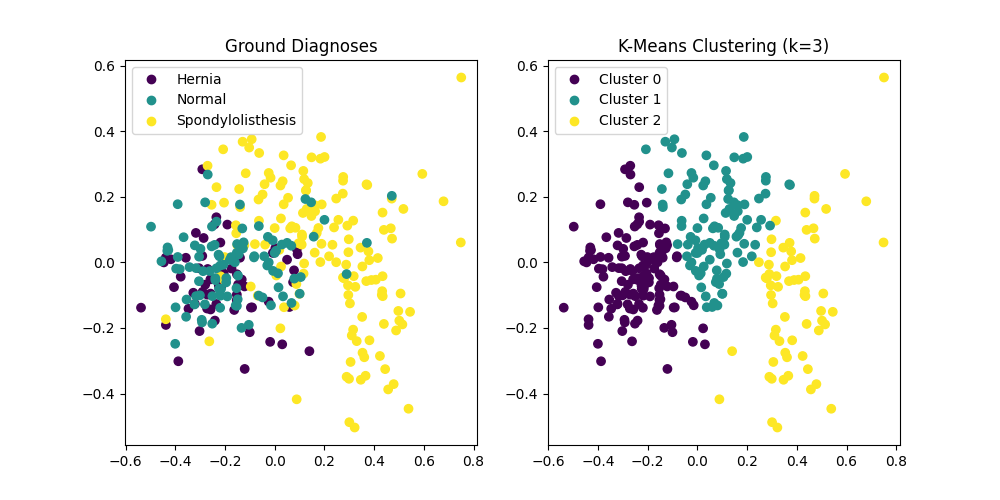
\includegraphics[width=17cm]{./assets/ex3-plot.png}
            \caption{Projected data}
            \label{fig:PartII-ex3}
        \end{figure}

    \item \textbf{Considering the results from questions (1) and (3), identify two ways on how clustering can
          be used to characterize the population of ill and healthy individuals.}

          \vskip 0.3cm
          Raquel
\end{enumerate}
\end{document}
